\chapter{Language Usage Tutorial}

This will cover the configuration of the user's environment and the usage of Extend's features.

\section{Setup}
The Extend compiler requires that the OCaml Language and LLVM be installed on the host machine. Development was done in a virtual machine running the 64-bit Ubuntu operating system. In order to quickly get Extend up and running, please use \underline{\href{https://courseworks2.columbia.edu/courses/10787/files/673708/download}{this virtual machine}}, which has been provided as part of the course.

	\medskip \noindent After booting up the virtual machine, clone the Extend git repository:

	\begin{lstlisting}
		git clone https://github.com/ExtendLang/Extend.git
	\end{lstlisting}

\section{Compiling and Running Extend Code}
To build the Extend compiler, the first steps are the following.

	\begin{lstlisting}
cd Extend/
make
	\end{lstlisting}

	\medskip \noindent
	If this does not successfully build, run \texttt{eval `opam config env`}, which should configure the environment to use OPAM packages. Alternatively, add this command to your bash profile.

	 \medskip \noindent
	 After running \texttt{make}, you should see a \texttt{main.byte} file. To compile and run an Extend program, we have provided a shell script to simplify the process for the user:

	\begin{lstlisting}
	./compile.sh example_source_file.xtnd
	\end{lstlisting}

	\medskip \noindent
	This should produce an \texttt{out} file. Running \texttt{./out} should successfully execute the program.
\section{Illustrating the Benefits of Extend}
Spreadsheet applications require the use of manual input in order to apply the same calculation to a different set of data. Extend aims to tackle this problem by offering portability. Below is an example of a spreadsheet user calculating the unit vector of a column vector:

\begin{center}
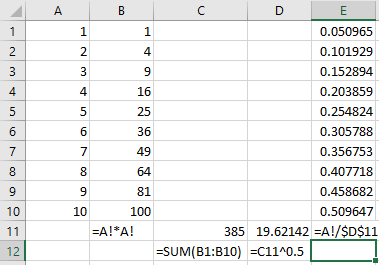
\includegraphics[width=7cm]{img/unitvector.png}
\end{center}

\medskip \noindent The Excel user must manually input the data, and additionally make space for the intermediate steps of the calculation. As the data becomes more diverse and the problem becomes more complicated, more work is required. Below is the equivalent function in Extend, written to work on any column vector that is passed in:

\begin{lstlisting}
	normalize_column_vector([m,1] arg) {
	  [m,1] squared_lengths := #arg * #arg, normalized := #arg / vector_norm;
	  vector_norm := sqrt(sum(squared_lengths));
	  return normalized;
	}
\end{lstlisting}

\medskip \noindent Another particularly interesting example is concatenating a row of strings of variable length with a common delimiter. This in an entirely manual operation for the spreadsheet user; a step-by-step attempt is shown below.

\begin{center}
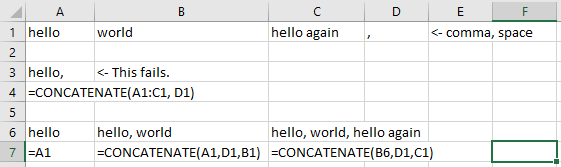
\includegraphics[width=9cm,height=3cm]{img/concatenation.png}
\end{center}

\medskip \noindent Performing a delimiter 'join' like the above can be performed in a simple program in Extend without knowing the size of the row.

\begin{lstlisting}
main(args){
	bar := {"Hello", "Goodbye", "Hello Again"};
	str := ", ";
	return foo(bar, str);\\ prints "Hello, Goodbye, Hello Again"
}

foo([1,n] colrange, str){
	[1,n] baz;
	baz[0,0] = #colrange;
	baz[0,1:] = baz[0,[-1]] + str + colrange[0,[0]];
	return print_endline(baz[0,-1]);
}
\end{lstlisting}

\medskip \noindent As evidenced above by simple examples, Extend offers flexibility that is significantly harder to achieve with conventional spreadsheet applications. As the nature of the data grows in complexity and variety, Extend's value increases.

\section{Writing Extend Code - The Basics}
Extend code can be written in a file that contains the conventional \texttt{.xtnd} extension. It consists of optional import statements and global variables, and an optional set of functions. Runnable Extend programs must contain a \texttt{main} function, and other functions can be written into the program as well.

\medskip \noindent
Below is a short tour of the features of Extend. More detail can be found in the next chapter - the Language Reference Manual.

	\subsection{Functions}
	Functions are commonplace in Extend. They are declared with the syntax \texttt{function\_name([optional\_dimensions] function\_arguments)\{...\}}. Below is the syntax of the \texttt{main} function, which is needed to run Extend code, within a simple Extend program.

	\begin{lstlisting}
	main(args){
			return 0;
	}
	\end{lstlisting}
	% Perhaps a more informative program - but not too difficult.

	\medskip \noindent
 	The return type of a function is a \textbf{range} of flexible size. \textbf{Ranges} will be discussed in a later section of this chapter. A function is composed of a series of statements, concluding with the return statement.
	Note that the \textbf{return} statement is always the last statement in the function.

		\subsubsection{Function Parameters}
		Function parameters consist of zero or more ranges, signed with an optional dimension. If the arguments have been written with dimensions, those dimensions will be verified at runtime.
		\begin{lstlisting}
			foo([m,n] arg){
				return m * n; \\ m and n initialized through arg1
			}

			bar([1,1] arg){
				return 0; \\ 1 by 1 ranges should be primitive data types. If arg is not, a runtime error will be thrown
			}
		\end{lstlisting}

	\subsection{Adjusting to Extend's Declarative Behavior}
	An important aspect of Extend is that the concept of a simple statement, barring the \texttt{return} statement, does not exist. In an Extend function, there are only declarations, formula assignments, and a return expression. As a declarative language, Extend examines the \texttt{return} statement, and simply evaluates the lines that will help get that return value. All other lines are ignored.

	\medskip \noindent The below Extend source file will not compile.

	\begin{lstlisting}
		main(args){
			foo := "Hello World!";
			print_endline(foo);\\ Cannot have this line. Must equal some formula.
			return foo;
		}
	\end{lstlisting}

	\medskip \noindent The below file compiles and prints successfully.

	\begin{lstlisting}
		main(args){
			foo := "Hello World!";
			return print_endline(foo); \\ print_endline is required in the return statement, and therefore runs
		}
	\end{lstlisting}

	\medskip \noindent As illustrated, Extend only evaluates what is needed to produce the value required by \texttt{return}. Any non-essential declarations or formula assignments will be ignored by the program. If the user attempts to write statements like \texttt{print\_endline("Hello")} by itself, the program will not compile.

	\subsection{Primitive Data Types}
	Extend has three primitive data types: Numbers, Strings, and \texttt{empty}. An example of each is shown below.

	\begin{lstlisting}
		bar := 5; \\ Assigns bar to a number
		foo := "Hello World"; \\ Assigns foo to a string
		bar = empty; \\ Reassigns bar to empty
	\end{lstlisting}

	\medskip \noindent
	\textbf{Note} that we declare a variable and assign it a value together with \texttt{:=}. If the variable already exists, \texttt{=} will suffice.
	More information about Extend's primitive data types can be found in the Language Reference Manual.

		\subsubsection{The typeof function}
		Extend offers a \texttt{typeof(expr)} function, which takes and expression and returns Number, String, Range, or Empty.

	\subsection{Operators}
	Extend includes a comprehensive set of operators. Each category is listed in order of precedence. A more detailed explanation of each operator can be found in the Language Reference Manual.

		\subsubsection{Arithmetic Operators}
			\begin{itemize}
				\item Unary Operations: \texttt{-}
				\item Binary Operations: \texttt{**, *, /, \%, +, -}
			\end{itemize}

		\subsubsection{Bitwise Operators}
			\begin{itemize}
				\item Unary Operations: \texttt{\~}
				\item Binary Operations: \texttt{<<, >>, \&, |, \^}
			\end{itemize}

		\subsubsection{Boolean Operators}
			\begin{itemize}
				\item Unary Operations: \texttt{!}
				\item Binary Operations: \texttt{==, !=, <, >, <=, >=, \&\&, ||}
			\end{itemize}

		\subsubsection{String Concatenation}
		Note that the \texttt{+} symbol can be used to perform concatenation between two strings.

		\begin{lstlisting}
			"Hello " + "World\n"
		\end{lstlisting}

	\subsection{Conditionals}
	There are two types of conditionals: the ternary conditional and a \texttt{switch} expression.

		\subsubsection{The Ternary Conditional}
		The two ways to write the ternary condition are as follows: \newline \newline
		\texttt{condition ? expr\_if\_true : expr\_if\_false} \newline \newline
		or: \newline \newline
		\texttt{if(conditional, expr\_if\_true, expr\_if\_false)}

		\subsubsection{The Switch Expression}
		Below is an example of the switch case used in a function:

		\begin{lstlisting}
			switch_func(foo){
				return switch(foo){
					case 1: "Hello, one!";
					case 2: "Hello, two!";
					default: "Hello?";
				};
			}
		\end{lstlisting}

	\subsection{Ranges}
	In Extend, \texttt{variables} are composed of cells. Under the hood, each cell points to a structure that may contain either primitive values or another \texttt{range}. This range can point to anonymous variables that are dereferenced in the aforementioned fashion as many times as needed to reveal the primitive value of the cell.
	\newline \newline
	Ranges are an incredibly important aspect of Extend. A range is composed of rows and columns of values.
	Each value can contain a formula that can evaluate to another range or one of the aforementioned three data types - number, string, or \texttt{empty}. Note that \textbf{1 by 1} ranges are automatically dereferenced to their contents in Extend.

	\begin{lstlisting}
		[1,2] foo; \\ Declares range of dimensions 1 by 2
		[1,3] bar := 4; \\ Declares range of dimensions 1 by 3, and assigns each cell to 4
	\end{lstlisting}

	\medskip \noindent
	Ranges can also be declared as range literals. Rows are delineated by \texttt{;} and columns by \texttt{,}.

	\begin{lstlisting}
		foo := {"Hello", 1, 2; 3, 4, 5; 6, 7, 8} \\ Three rows, three columns.
	\end{lstlisting}

		\subsubsection{Range Slicing \& Selection}
		Python-style array-slicing syntax can be applied to ranges, which will return a subrange based on either absolute or relative indexing. All indices are zero-based.

		\begin{lstlisting}
			foo[0,2] \\ The cell in the first row, third column
			foo[0,:] \\ The range of cells in the first row
			foo[0,[1]] \\ The range in the column that is 1 column right of the left-hand-side cell.
			foo[,] \\ Cell in first row, first column if 1 by 1. If not, then relative first row and relative first column
		\end{lstlisting}

		\medskip \noindent
		More examples and detail can be found in the next chapter.

		\subsubsection{The Hash Operator}
		A common case for ranges in Excel is to perform calculations on specific cells. For example, \texttt{foo[,]} is commonly used to retrieve the cell that is being calculated on.
		Since this is a popular use case, the \texttt{\#} operator will perform the same functionality.

		\subsubsection{Application on Ranges}
		Extend, in the vein of spreadsheets, allows the programmer to apply functions cell-wise on a range. Using the \texttt{\#} operator, we can perform cell-wise multiplication across two ranges.

		\begin{lstlisting}
			foo([m,n] arg1, [m.n] arg2){
				[m,n] bar := #arg1 * #arg2; \\ Multiplies the cell in arg1 with the corresponding cell in arg2.
				return bar;
			}
		\end{lstlisting}

		\medskip \noindent
		This is an incredibly powerful aspect of Extend. Make sure to study it well!

		\subsubsection{Range Attribute Functions}
		Extend has the \texttt{row()} and \texttt{column()} functions, which respectively return the row and column of the cell that is being calculated at that point in time.
		There is also a \texttt{size(expr)} function, which returns a 1 by 2 range; the first cell contains the number of rows, and the second cell contains the number of columns.

	\subsection{Precedence Expressions}
	Precedence Expressions are used to force the evaluation of one expression before another. This is used when the order of operation is required for functions with side effects, such as the ones housed in Extend's standard library.
	The \texttt{->} operator is used to denote precedence.

	\begin{lstlisting}
		return print_func(4) -> 0; \\ print_func prints 4 to stdout before returning 0
	\end{lstlisting}

	\subsection{Import Statements}
	In Extend, you can import other Extend files at the top of your program via relative directory path. The use case is below:

	\begin{lstlisting}
		import "../programs/helloworld.xtnd"
	\end{lstlisting}

\section{Standard Library Functions}
Extend offers an assortment of standard library functions. Extend imports \texttt{stdlib.xtnd}, which has aggregated all the standard library functions for the user's disposal.

\medskip \noindent
While their usage will be covered in more length in the Language Reference Manual, here are some of the more useful standard library functions to remember.
	\subsection{Basic Functions}
		\subsubsection{The toString() Function}
		The \texttt{toString()} function takes a 1 by 1 range and renders its value as a string. This will return one of the primitive data types.

		\begin{lstlisting}
			return "Hello " + toString(14); \\ "Hello 14"
		\end{lstlisting}

		\subsubsection{Math Functions}
		Borrowing from C's standard library math functions, Extend offers: \texttt{sin, cos, tan, acos, asin, atan, sinh, cosh, tanh, exp, log, log10, sqrt, ceil, fabs} and \texttt{floor}.

		\begin{lstlisting}
			main(args){
				bar := sqrt(16);
				return write(STDOUT, toString(bar)) -> 0; \\ Prints 4 to stdout
			}
		\end{lstlisting}

	\subsection{File I/O}
	Extend has \texttt{open, close, read, and write} functions to interact with files. Usage is as follows:

	\begin{lstlisting}
		main(args){
		  return write(STDOUT, read(open("test_file.txt", "r"),5)) -> 0; \\ Writes 5 characters from test_file.txt to stdout
		}
	\end{lstlisting}

	\subsection{Plotting}
	Extend also offers the ability to export plots to a PNG file with the \texttt{plot} function.

	\begin{lstlisting}
		TODO: Demonstrate usage here.
	\end{lstlisting}
